

\actTitle{Worksheet 1.6B}


\noindent \textbf{Instructions:}  Work together in groups of  3 or 4 to complete the following problems.




\begin{enumerate}
\item Use the graph of $y=f(x)$ below to graph the given functions.
\begin{enumerate}
\item $\displaystyle y=\frac{1}{3}f(x)$
\item $y=3f(x)$
\item $y=f(2x)$
\item $\displaystyle y=f(\frac{1}{2}x)$
\end{enumerate}



\begin{center}
	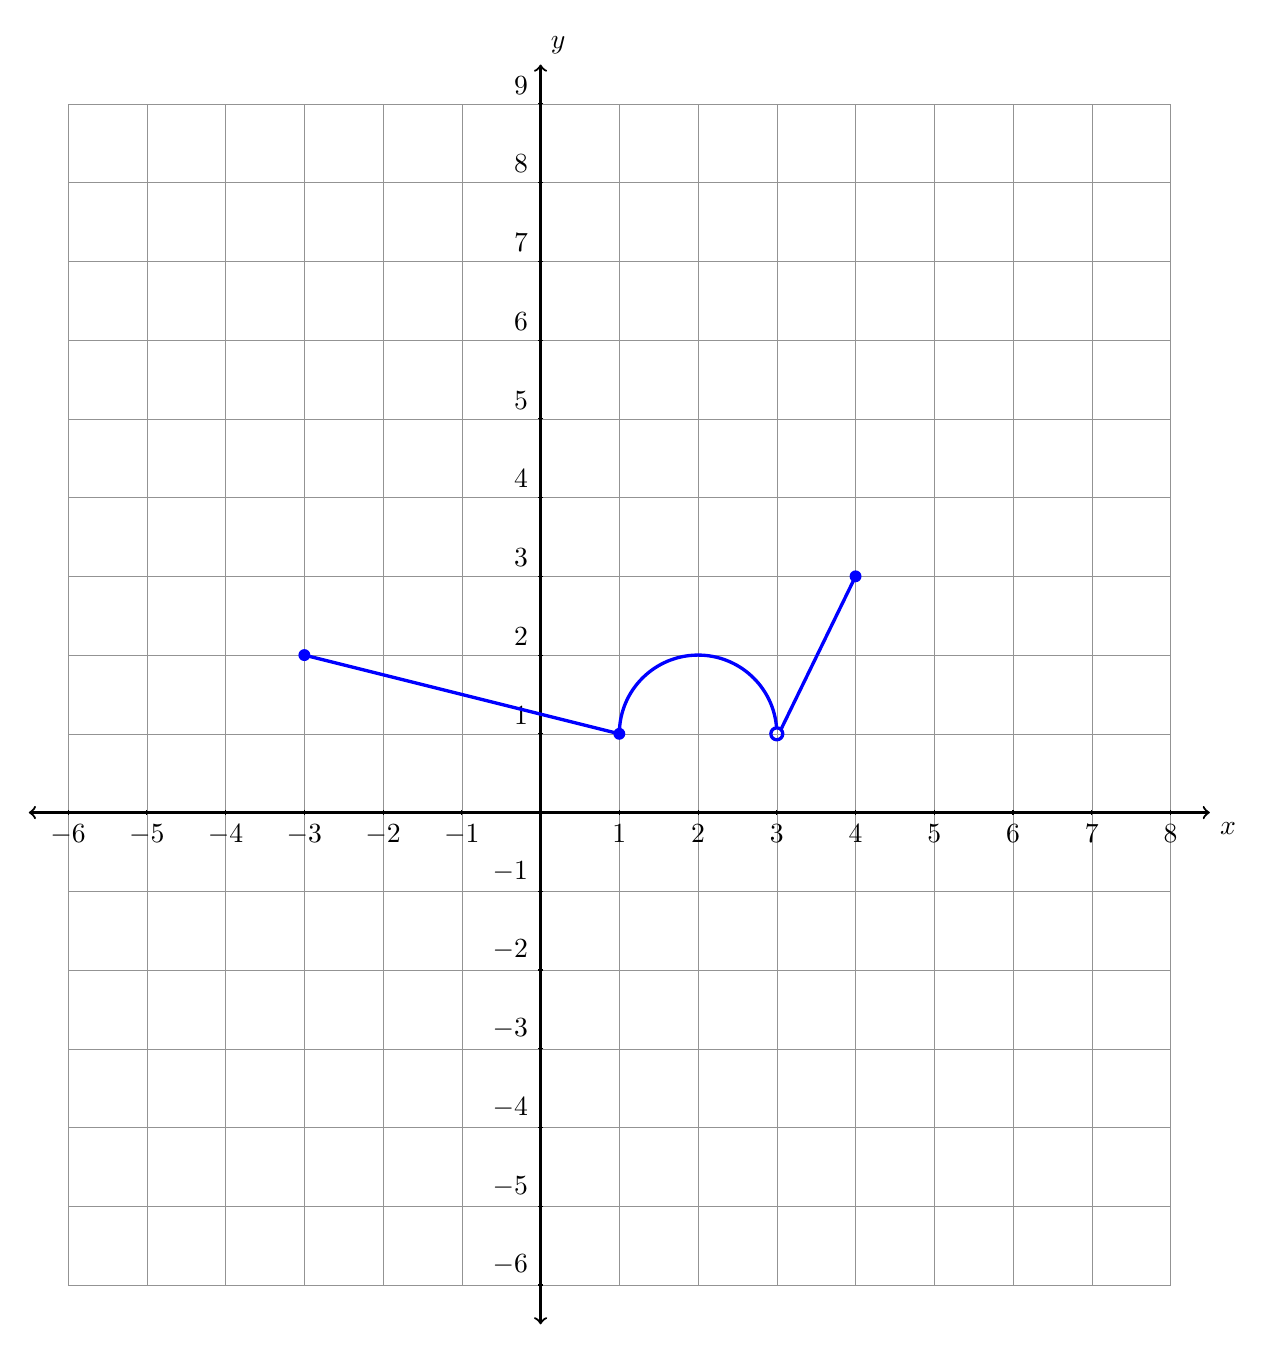
\begin{tikzpicture}[y=1cm, x=1cm,font=\sffamily,
	mydot/.style={
    circle,
    fill=white,
    draw,
    outer sep=0pt,
    inner sep=1.5pt
  }]
    %% Add a grid
    \draw[step = 1, gray, very thin,opacity=0.85] (-6, -6) grid (8, 9);
 	%% Draw the axes
	\draw[thick,<->] (-6.5,0) -- coordinate (x axis mid) (8.5,0) node[anchor = north west] {$x$};
    \draw[thick,<->] (0,-6.5) -- coordinate (y axis mid) (0,9.5) node[anchor = south west] {$y$};
    %% Label the y axis
    \foreach \y in {-6,...,-1,1,2,...,9} {
      \draw (1pt, \y) -- (-1pt, \y) node[anchor = south east] {$\y$};
    }
    %% Label the x axis
    \foreach \x in {-6,...,-1,1,2,...,8} {
      \draw (\x,1pt) -- (\x,-1pt) node[anchor = north] {$\x$};
    }
    %% Draw the function.
    \begin{scope}
         \draw[very thick,blue] (-3,2) -- (1,1);
         \draw[very thick,blue] (3.05,1.05) -- (4,3);
    %semi-circle
         \draw[very thick, blue] (1,1) arc [radius=1, start angle=180, end angle= 5];
     %parabola
     %    \draw[ultra thick, black, domain=-5:0] plot (\x, {(-0.2)*(\x-5)*(\x+5)});
     %dots
         \fill[blue] (-3, 2) circle[radius=0.5ex];
         \fill[blue] (1,1) circle[radius=0.5ex];
         \fill[blue] (4,3) circle[radius=0.5ex];
         \draw[very thick, blue] (3,1) circle[radius=0.5ex];


    \end{scope}

    %%\node[above=0.1cm] at (-2,2 )   {\nextXValue};

  \end{tikzpicture}
\end{center}

\newpage

\item Use the graph of $y=f(x)$ below to graph the given functions.
\begin{enumerate}
\item $y=-f(x)$
\item $y=f(-x)$
\item $y=-f(-x)$
\end{enumerate}



\begin{center}
	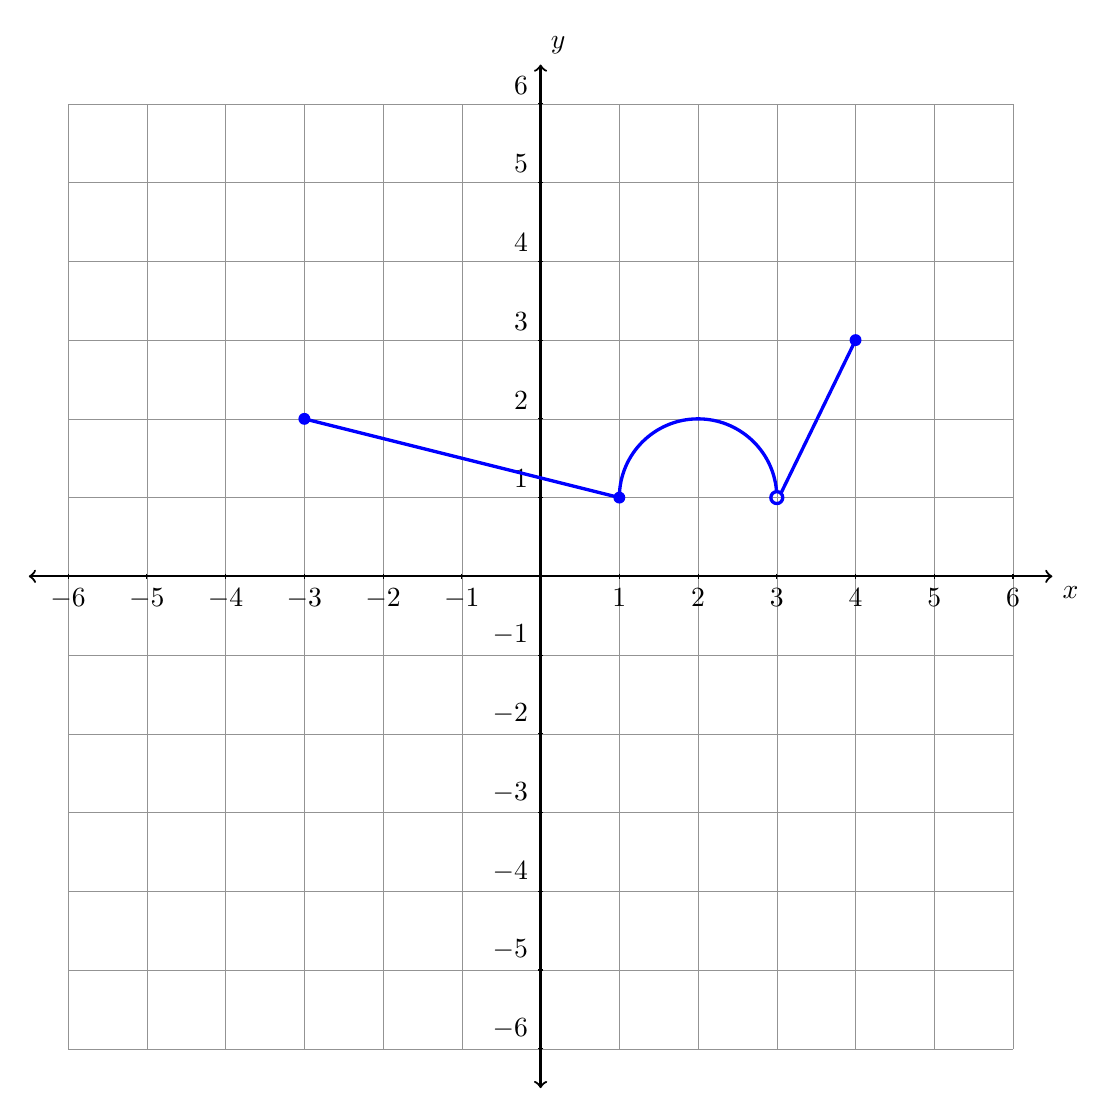
\begin{tikzpicture}[y=1cm, x=1cm,font=\sffamily,
	mydot/.style={
    circle,
    fill=white,
    draw,
    outer sep=0pt,
    inner sep=1.5pt
  }]
    %% Add a grid
    \draw[step = 1, gray, very thin,opacity=0.85] (-6, -6) grid (6, 6);
 	%% Draw the axes
	\draw[thick,<->] (-6.5,0) -- coordinate (x axis mid) (6.5,0) node[anchor = north west] {$x$};
    \draw[thick,<->] (0,-6.5) -- coordinate (y axis mid) (0,6.5) node[anchor = south west] {$y$};
    %% Label the y axis
    \foreach \y in {-6,...,-1,1,2,...,6} {
      \draw (1pt, \y) -- (-1pt, \y) node[anchor = south east] {$\y$};
    }
    %% Label the x axis
    \foreach \x in {-6,...,-1,1,2,...,6} {
      \draw (\x,1pt) -- (\x,-1pt) node[anchor = north] {$\x$};
    }
    %% Draw the function.
    \begin{scope}
         \draw[very thick,blue] (-3,2) -- (1,1);
         \draw[very thick,blue] (3.05,1.05) -- (4,3);
    %semi-circle
         \draw[very thick, blue] (1,1) arc [radius=1, start angle=180, end angle= 5];
     %parabola
     %    \draw[ultra thick, black, domain=-5:0] plot (\x, {(-0.2)*(\x-5)*(\x+5)});
     %dots
         \fill[blue] (-3, 2) circle[radius=0.5ex];
         \fill[blue] (1,1) circle[radius=0.5ex];
         \fill[blue] (4,3) circle[radius=0.5ex];
         \draw[very thick, blue] (3,1) circle[radius=0.5ex];


    \end{scope}

    %%\node[above=0.1cm] at (-2,2 )   {\nextXValue};

  \end{tikzpicture}
\end{center}

\newpage


\item Identify and sketch the \emph{parent} function of each of the following functions. \\
Then use the transformation rules to sketch their graphs.
\begin{itemize}

\item[(a)] $f(x)=\sqrt{2x+4}-1$, \hfill parent function:  \hfill \hfill

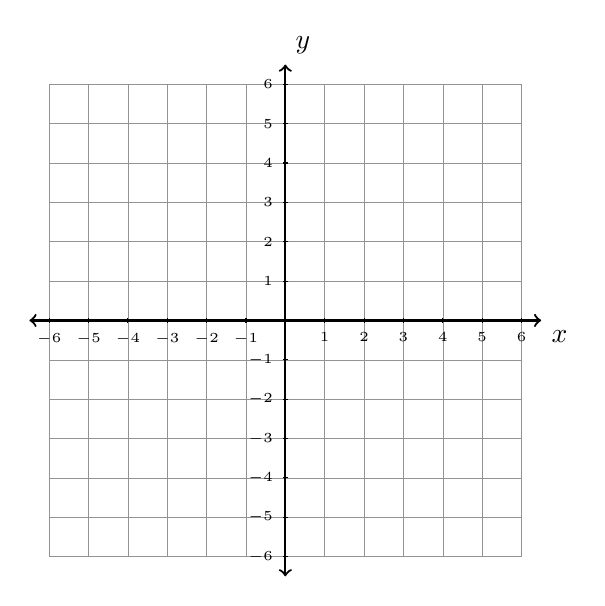
\begin{tikzpicture}[y=.5cm, x=.5cm,font=\sffamily,
	mydot/.style={
    circle,
    fill=white,
    draw,
    outer sep=0pt,
    inner sep=1.5pt
  }]
    %% Add a grid
    \draw[step = 1, gray, very thin,opacity=0.85] (-6, -6) grid (6, 6);
 	%% Draw the axes
	\draw[thick,<->] (-6.5,0) -- coordinate (x axis mid) (6.5,0) node[anchor = north west] {$x$};
    \draw[thick,<->] (0,-6.5) -- coordinate (y axis mid) (0,6.5) node[anchor = south west] {$y$};
    %% Label the y axis
    \foreach \y in {-6,...,-1,1,2,...,6} {
      \draw (1pt, \y) -- (-1pt, \y) node[anchor =  east] {\tiny$\y$};
    }
    %% Label the x axis
    \foreach \x in {-6,...,-1,1,2,...,6} {
      \draw (\x,1pt) -- (\x,-1pt) node[anchor = north] {\tiny$\x$};
    }
    %% Draw the function.
 %   \begin{scope}
 %        \draw[very thick,black] (-3,2) -- (1,1);
 %        \draw[very thick,black] (3.05,1.05) -- (4,3);
    %semi-circle
  %       \draw[very thick, black] (1,1) arc [radius=1, start angle=180, end angle= 5];
     %parabola
     %    \draw[ultra thick, black, domain=-5:0] plot (\x, {(-0.2)*(\x-5)*(\x+5)});
     %dots
     %  \fill[black] (-3, 2) circle[radius=0.5ex];
     %   \fill[black] (1,1) circle[radius=0.5ex];
     %    \fill[black] (4,3) circle[radius=0.5ex];
     %     \draw[very thick, black] (3,1) circle[radius=0.5ex];


   % \end{scope}

    %%\node[above=0.1cm] at (-2,2 )   {\nextXValue};

  \end{tikzpicture}

\vspace{0.5in}


\item[(b)] $g(x)=(-x+1)^3$ , \hfill parent function:  \hfill \hfill

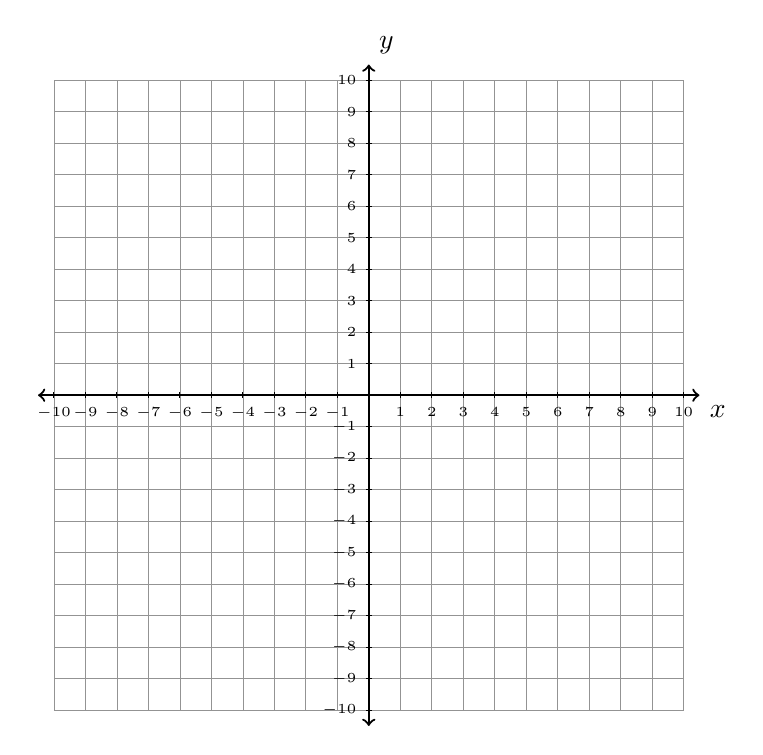
\begin{tikzpicture}[y=.4cm, x=.4cm,font=\sffamily,
	mydot/.style={
    circle,
    fill=white,
    draw,
    outer sep=0pt,
    inner sep=1.5pt
  }]
    %% Add a grid
    \draw[step = 1, gray, very thin,opacity=0.85] (-10, -10) grid (10, 10);
 	%% Draw the axes
	\draw[thick,<->] (-10.5,0) -- coordinate (x axis mid) (10.5,0) node[anchor = north west] {$x$};
    \draw[thick,<->] (0,-10.5) -- coordinate (y axis mid) (0,10.5) node[anchor = south west] {$y$};
    %% Label the y axis
    \foreach \y in {-10,...,-1,1,2,...,10} {
      \draw (1pt, \y) -- (-1pt, \y) node[anchor =  east] {\tiny$\y$};
    }
    %% Label the x axis
    \foreach \x in {-10,...,-1,1,2,...,10} {
      \draw (\x,1pt) -- (\x,-1pt) node[anchor = north] {\tiny$\x$};
    }
    %% Draw the function.
 %   \begin{scope}
 %        \draw[very thick,black] (-3,2) -- (1,1);
 %        \draw[very thick,black] (3.05,1.05) -- (4,3);
    %semi-circle
  %       \draw[very thick, black] (1,1) arc [radius=1, start angle=180, end angle= 5];
     %parabola
     %    \draw[ultra thick, black, domain=-5:0] plot (\x, {(-0.2)*(\x-5)*(\x+5)});
     %dots
     %  \fill[black] (-3, 2) circle[radius=0.5ex];
     %   \fill[black] (1,1) circle[radius=0.5ex];
     %    \fill[black] (4,3) circle[radius=0.5ex];
     %     \draw[very thick, black] (3,1) circle[radius=0.5ex];


   % \end{scope}

    %%\node[above=0.1cm] at (-2,2 )   {\nextXValue};

  \end{tikzpicture}


\newpage

\item[(c)] $h(x)=\sqrt[3]{8x}-2$  , \hfill parent function:  \hfill \hfill

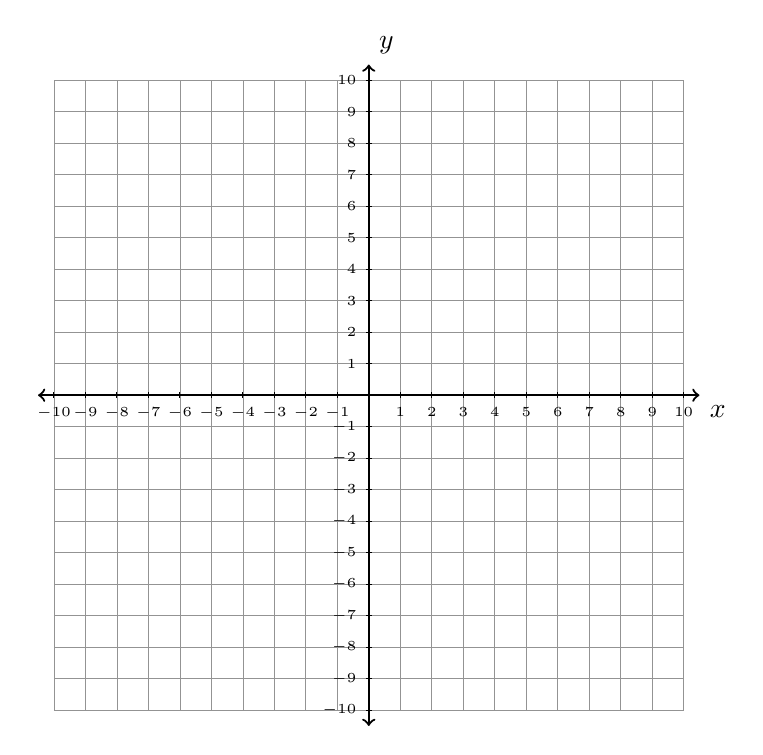
\begin{tikzpicture}[y=.4cm, x=.4cm,font=\sffamily,
	mydot/.style={
    circle,
    fill=white,
    draw,
    outer sep=0pt,
    inner sep=1.5pt
  }]
    %% Add a grid
    \draw[step = 1, gray, very thin,opacity=0.85] (-10, -10) grid (10, 10);
 	%% Draw the axes
	\draw[thick,<->] (-10.5,0) -- coordinate (x axis mid) (10.5,0) node[anchor = north west] {$x$};
    \draw[thick,<->] (0,-10.5) -- coordinate (y axis mid) (0,10.5) node[anchor = south west] {$y$};
    %% Label the y axis
    \foreach \y in {-10,...,-1,1,2,...,10} {
      \draw (1pt, \y) -- (-1pt, \y) node[anchor =  east] {\tiny$\y$};
    }
    %% Label the x axis
    \foreach \x in {-10,...,-1,1,2,...,10} {
      \draw (\x,1pt) -- (\x,-1pt) node[anchor = north] {\tiny$\x$};
    }
    %% Draw the function.
 %   \begin{scope}
 %        \draw[very thick,black] (-3,2) -- (1,1);
 %        \draw[very thick,black] (3.05,1.05) -- (4,3);
    %semi-circle
  %       \draw[very thick, black] (1,1) arc [radius=1, start angle=180, end angle= 5];
     %parabola
     %    \draw[ultra thick, black, domain=-5:0] plot (\x, {(-0.2)*(\x-5)*(\x+5)});
     %dots
     %  \fill[black] (-3, 2) circle[radius=0.5ex];
     %   \fill[black] (1,1) circle[radius=0.5ex];
     %    \fill[black] (4,3) circle[radius=0.5ex];
     %     \draw[very thick, black] (3,1) circle[radius=0.5ex];


   % \end{scope}

    %%\node[above=0.1cm] at (-2,2 )   {\nextXValue};

  \end{tikzpicture}
  

\vspace{1in}

\item[(d)] $k(x)=3-\displaystyle\frac{1}{(x+2)}$  , \hfill parent function:  \hfill \hfill

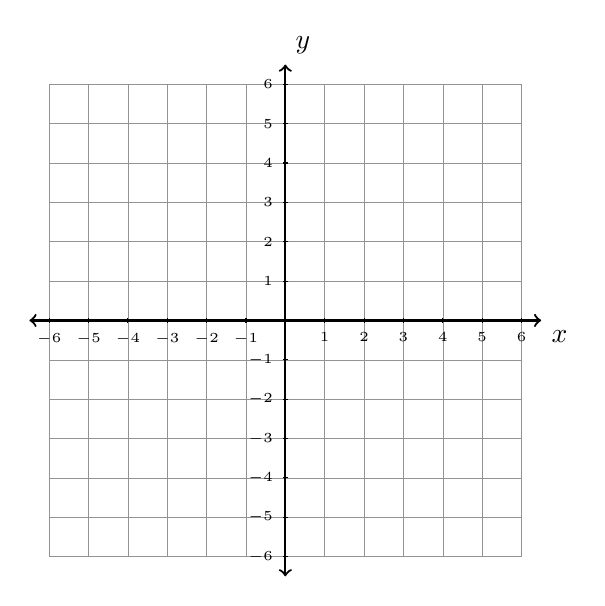
\begin{tikzpicture}[y=.5cm, x=.5cm,font=\sffamily,
	mydot/.style={
    circle,
    fill=white,
    draw,
    outer sep=0pt,
    inner sep=1.5pt
  }]
    %% Add a grid
    \draw[step = 1, gray, very thin,opacity=0.85] (-6, -6) grid (6, 6);
 	%% Draw the axes
	\draw[thick,<->] (-6.5,0) -- coordinate (x axis mid) (6.5,0) node[anchor = north west] {$x$};
    \draw[thick,<->] (0,-6.5) -- coordinate (y axis mid) (0,6.5) node[anchor = south west] {$y$};
    %% Label the y axis
    \foreach \y in {-6,...,-1,1,2,...,6} {
      \draw (1pt, \y) -- (-1pt, \y) node[anchor =  east] {\tiny$\y$};
    }
    %% Label the x axis
    \foreach \x in {-6,...,-1,1,2,...,6} {
      \draw (\x,1pt) -- (\x,-1pt) node[anchor = north] {\tiny$\x$};
    }
    %% Draw the function.
 %   \begin{scope}
 %        \draw[very thick,black] (-3,2) -- (1,1);
 %        \draw[very thick,black] (3.05,1.05) -- (4,3);
    %semi-circle
  %       \draw[very thick, black] (1,1) arc [radius=1, start angle=180, end angle= 5];
     %parabola
     %    \draw[ultra thick, black, domain=-5:0] plot (\x, {(-0.2)*(\x-5)*(\x+5)});
     %dots
     %  \fill[black] (-3, 2) circle[radius=0.5ex];
     %   \fill[black] (1,1) circle[radius=0.5ex];
     %    \fill[black] (4,3) circle[radius=0.5ex];
     %     \draw[very thick, black] (3,1) circle[radius=0.5ex];


   % \end{scope}

    %%\node[above=0.1cm] at (-2,2 )   {\nextXValue};

  \end{tikzpicture}
  
  

\end{itemize}



\newpage


%\item  For this problem, let $f(x)=\sqrt[3]{x}$.
%
%\begin{enumerate}
%\item Graph $f(x)=\sqrt[3]{x}$.  Then determine the domain and range of $f(x)$.\\
%\begin{tikzpicture}[y=.5cm, x=0.5cm,font=\sffamily]
%    %% ticks
%    \draw[step = 1, gray] (-11,-11) grid (11,11);
%    %% axis
%    \draw[thick,->] (-11.5,0) -- coordinate (x axis mid) (11,0) node[anchor = north west] {$x$};
%    \draw[thick,->] (0,-11.5) -- coordinate (y axis mid) (0,11) node[anchor = north east] {$y$};
%    \foreach \y in {-6,-5,...,-1,1,2,...,6} {
%      \draw (2pt, \y) -- (-2pt, \y);
%    }
%    \foreach \x in {-6,-5,...,-1,1,2,...,6} {
%      \draw (\x,2pt) -- (\x,-2pt);
%    }
%
%  \end{tikzpicture}
%
%\item Use part (a) to graph $g(x)=5\sqrt[3]{x}$ above.  \vfill
%\item Use part (a) to graph $h(x)=\sqrt[3]{2x}$ above.  \vfill
%\item Use part (a) to graph $\displaystyle j(x)=\sqrt[3]{\frac{1}{4}x}$ above.  \vfill
%\end{enumerate}
%
%
%
%
%\newpage
%
%\item  For this problem, let $f(x)=|x|$.
%
%\begin{enumerate}
%\item Graph $f(x)=|x|$.  Then determine the domain and range of $f(x)$.\\
%\begin{tikzpicture}[y=.5cm, x=0.5cm,font=\sffamily]
%    %% ticks
%    \draw[step = 1, gray] (-11,-11) grid (11,11);
%    %% axis
%    \draw[thick,->] (-11.5,0) -- coordinate (x axis mid) (11,0) node[anchor = north west] {$x$};
%    \draw[thick,->] (0,-11.5) -- coordinate (y axis mid) (0,11) node[anchor = north east] {$y$};
%    \foreach \y in {-6,-5,...,-1,1,2,...,6} {
%      \draw (2pt, \y) -- (-2pt, \y);
%    }
%    \foreach \x in {-6,-5,...,-1,1,2,...,6} {
%      \draw (\x,2pt) -- (\x,-2pt);
%    }
%
%  \end{tikzpicture}
%
%\item Use part (a) to graph $g(x)=-|x|$ above.  
%\vfill
%\item Use part (a) to graph $h(x)=|-x|$ above.  
%\vfill
%\item Use part (a) to graph $j(x)=-|x|+2$ above.  
%\vfill
%\end{enumerate}
%
%
%\newpage
%


\item Write a function $f(x)$ based on the given parent function and transformations in the given order.
\begin{enumerate}
\item $g(x)=x^2$ 
\begin{enumerate}
\item Shift 4 units to the left.
\item Reflect across the $y$-axis.
\item Shift upward 2 units.
\end{enumerate}

\vspace{1in}


\item $g(x)=\sqrt{x}$
\begin{enumerate}
\item Shift 1 unit to the left.
\item Stretch horizontally by a factor of 4.
\item Reflect across the $x$-axis.
\end{enumerate}

\vspace{1in}

\item $\displaystyle g(x)=\frac{1}{x}$
\begin{enumerate}
\item Stretch vertically by a factor of 2.
\item Reflect across the $x$-axis.
\item Shift downward 3 units.
\end{enumerate}

\vspace{1in}

\item $\displaystyle g(x)=|x|$
\begin{enumerate}
\item Shift 3 units to the right.
\item Shrink horizontally by a factor of $\displaystyle \frac{1}{3}$.
\item Reflect across the $y-axis$.
\end{enumerate}

\vspace{1in}

\end{enumerate}

\vfill
\newpage


\item Use transformations on the basic parent functions to write an equation $y=f(x)$ that would produce the given graph.

\begin{description}
	\item[(a)]\ 
	
\begin{center}
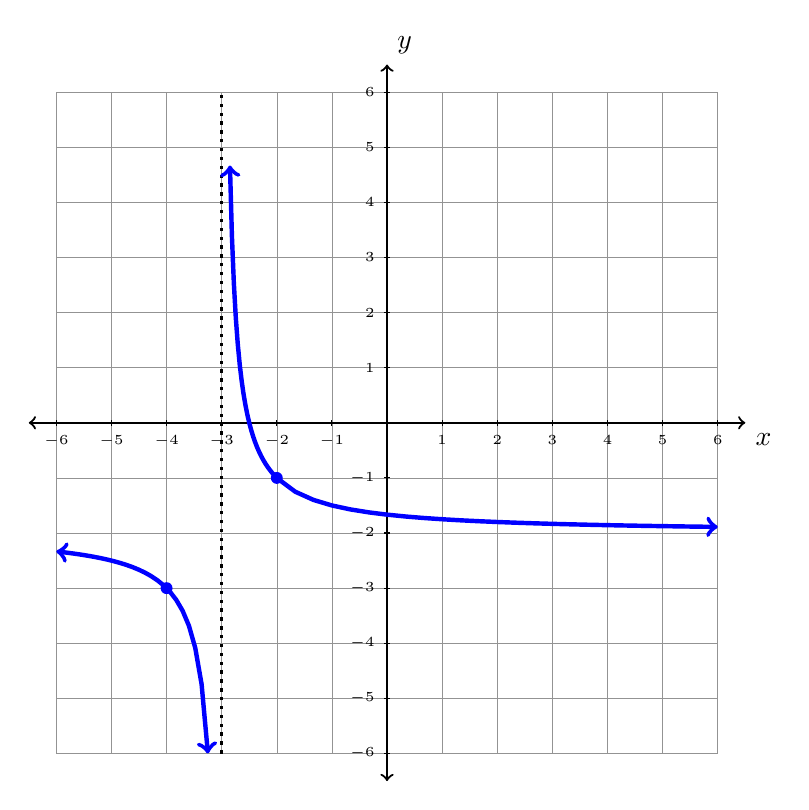
\begin{tikzpicture}[y=.7cm, x=.7cm,font=\sffamily,
	mydot/.style={
    circle,
    fill=white,
    draw,
    outer sep=0pt,
    inner sep=1.5pt
  }]
    %% Add a grid
    \draw[step = 1, gray, very thin,opacity=0.85] (-6, -6) grid (6, 6);
 	%% Draw the axes
	\draw[thick,<->] (-6.5,0) -- coordinate (x axis mid) (6.5,0) node[anchor = north west] {$x$};
    \draw[thick,<->] (0,-6.5) -- coordinate (y axis mid) (0,6.5) node[anchor = south west] {$y$};
    %% Label the y axis
    \foreach \y in {-6,...,-1,1,2,...,6} {
      \draw (1pt, \y) -- (-1pt, \y) node[anchor =  east] {\tiny$\y$};
    }
    %% Label the x axis
    \foreach \x in {-6,...,-1,1,2,...,6} {
      \draw (\x,1pt) -- (\x,-1pt) node[anchor = north] {\tiny$\x$};
    }
    %% Draw the function.
   \begin{scope}
         \draw[very thick,  dotted, black] (-3,-6) -- (-3,6);
 %        \draw[very thick,black] (3.05,1.05) -- (4,3);
    %semi-circle
  %       \draw[very thick, black] (1,1) arc [radius=1, start angle=180, end angle= 5];
     %function
         \draw[ultra thick, blue, <->, domain=-6:-3.25] plot (\x, {(\x + 3)^(-1)-2});
         \draw[ultra thick, blue, <-, domain=-2.85:-2] plot (\x, {(\x + 3)^(-1)-2});
         \draw[ultra thick, blue, ->, domain=-2:6] plot (\x, {(\x + 3)^(-1)-2});
     %dots
      \fill[blue] (-4, -3) circle[radius=0.5ex];
      \fill[blue] (-2,-1) circle[radius=0.5ex];
     %    \fill[black] (4,3) circle[radius=0.5ex];
     %     \draw[very thick, black] (3,1) circle[radius=0.5ex];


    \end{scope}

    %%\node[above=0.1cm] at (-2,2 )   {\nextXValue};

  \end{tikzpicture}
  \end{center}

	\item[(b)]\ 

\begin{center}
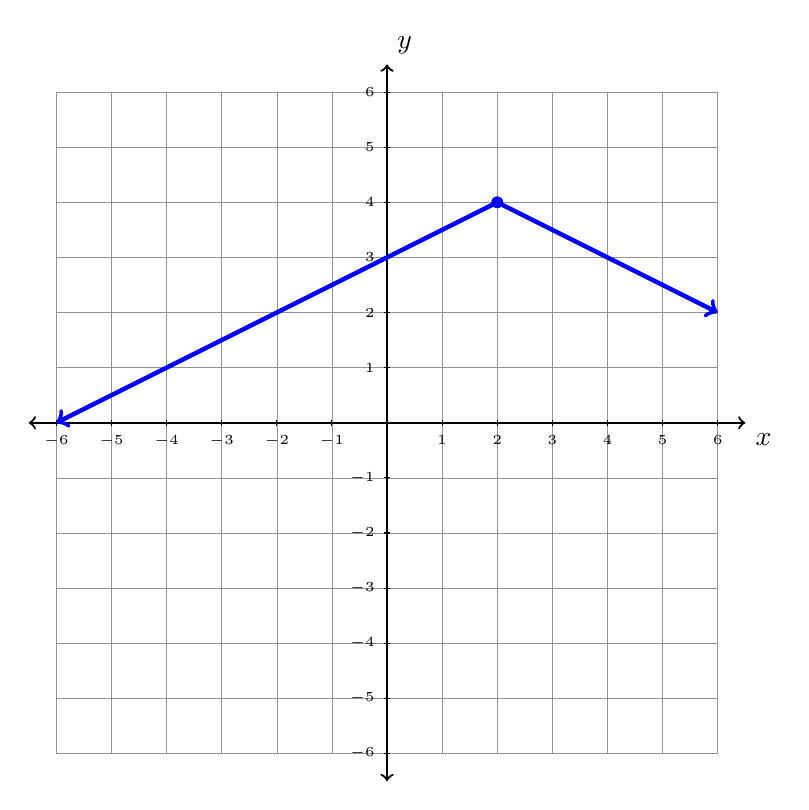
\begin{tikzpicture}[y=.7cm, x=.7cm,font=\sffamily,
	mydot/.style={
    circle,
    fill=white,
    draw,
    outer sep=0pt,
    inner sep=1.5pt
  }]
    %% Add a grid
    \draw[step = 1, gray, very thin,opacity=0.85] (-6, -6) grid (6, 6);
 	%% Draw the axes
	\draw[thick,<->] (-6.5,0) -- coordinate (x axis mid) (6.5,0) node[anchor = north west] {$x$};
    \draw[thick,<->] (0,-6.5) -- coordinate (y axis mid) (0,6.5) node[anchor = south west] {$y$};
    %% Label the y axis
    \foreach \y in {-6,...,-1,1,2,...,6} {
      \draw (1pt, \y) -- (-1pt, \y) node[anchor =  east] {\tiny$\y$};
    }
    %% Label the x axis
    \foreach \x in {-6,...,-1,1,2,...,6} {
      \draw (\x,1pt) -- (\x,-1pt) node[anchor = north] {\tiny$\x$};
    }
    %% Draw the function.
   \begin{scope}
  %       \draw[very thick,black] (-3,2) -- (1,1);
 %        \draw[very thick,black] (3.05,1.05) -- (4,3);
    %semi-circle
  %       \draw[very thick, black] (1,1) arc [radius=1, start angle=180, end angle= 5];
     %function
         \draw[ultra thick, blue, <-, domain=-6:2] plot (\x, {.5*\x+3});
         \draw[ultra thick, blue, ->, domain=2:6] plot (\x, {-.5*\x+5});
     %dots
       \fill[blue] (2, 4) circle[radius=0.5ex];
     %  \fill[black] (1,1) circle[radius=0.5ex];
     %    \fill[black] (4,3) circle[radius=0.5ex];
     %     \draw[very thick, black] (3,1) circle[radius=0.5ex];


    \end{scope}

    %%\node[above=0.1cm] at (-2,2 )   {\nextXValue};

  \end{tikzpicture}
  \end{center}
  
\end{description}


\item In words, explain how the graph of $\displaystyle f(x)=-\frac{1}{2}(x-4)^2+3$ is different from the graph of $g(x)=x^2$.  (Note:  List the transformations in the correct order.)


\vspace{2in}


\item If the point $(-2,5)$ is on the graph of $y=f(x)$, find the corresponding point on the graph of $y=-3f(7x)-4$

%\vspace{1.5in}
%
%\item Consider the parent function $f(x) = \sqrt x$.
%\begin{enumerate}
%	\item Write an equation for the function $g(x)$ that is obtained from $f(x)$ by first shifting left by 6, then compressing horizontally by a factor of 3.
%	\item Write an equation for the function $h(x)$ that is obtained from $f(x)$ by first compressing horizontally by a factor of 3, then shifting left by 2.
%	\item Compare your answers to part (a) and (b).  What does this tell you about the order in which we perform our transformations?
%\end{enumerate}


\end{enumerate}









